\documentclass{article}

% if you need to pass options to natbib, use, e.g.:
%     \PassOptionsToPackage{numbers, compress}{natbib}
% before loading neurips_2019

% ready for submission
% \usepackage{neurips_2019}

% to compile a preprint version, e.g., for submission to arXiv, add add the
% [preprint] option:
    % \usepackage[preprint]{neurips_2019}

% to compile a camera-ready version, add the [final] option, e.g.:
     \usepackage[final]{style}

% to avoid loading the natbib package, add option nonatbib:
%     \usepackage[nonatbib]{neurips_2019}

\usepackage[utf8]{inputenc} % allow utf-8 input
\usepackage[T1]{fontenc}    % use 8-bit T1 fonts
\usepackage{hyperref}       % hyperlinks
\usepackage{url}            % simple URL typesetting
\usepackage{booktabs}       % professional-quality tables
\usepackage{amsfonts}       % blackboard math symbols
\usepackage{subcaption}    % for subfigure environment
\usepackage{graphicx}       % for including graphics
\usepackage{float}          % for [H] float placement
\usepackage{nicefrac}       % compact symbols for 1/2, etc.
\usepackage{microtype}      % microtypography

\title{Robust Facial Emotion Recognition with Geometric Landmark Encoding and Continuous Facial Motions}

% The \author macro works with any number of authors. There are two commands
% used to separate the names and addresses of multiple authors: \And and \AND.
%
% Using \And between authors leaves it to LaTeX to determine where to break the
% lines. Using \AND forces a line break at that point. So, if LaTeX puts 3 of 4
% authors names on the first line, and the last on the second line, try using
% \AND instead of \And before the third author name.

\author{%
  Zhenghao Jin \\
  ECE \\
  \texttt{zhenghao@andrew.cmu.edu} \\
  \And
  Putian Wang \\
  ECE \\
  \texttt{putianw@andrew.cmu.edu} \\
  \And
  Veronica Zhao \\
  ECE \\
  \texttt{veronicz@andrew.cmu.edu} \\
}


\begin{document}

\maketitle

\section{Introduction}
Facial Emotion Recognition (FER) is a critical technology for next-generation human-computer interaction, enabling applications from adaptive tutoring systems to driver safety monitoring. For these systems to be effective, their predictions must be accurate and stable and reliable over time. However, real-world conditions present significant challenges: faces are often partially occluded, with constant variations in pose and lighting. Furthermore, existing models struggle to generalize across different individuals and often fail to capture subtle, low-amplitude expressions.

Although modern deep learning approaches have improved on the classical methods, they still have key limitations \cite{3}. CNN-based models, though powerful, often produce unstable frame-by-frame predictions and perform poorly when faced with data from new subjects or environments. Sequence models like RNNs can improve temporal consistency but at a high computational cost, making them less suitable for real-time applications.

Two primary gaps remain in current research: inadequate adaptation to the unique facial morphology of each input, and insufficient use of short-term facial dynamics, which are crucial for distinguishing near-neutral expressions. Our project directly addresses these gaps. We start with a naive initial experiment that utilizes only five landmarks and their relative distances to build a shallow Multi-Layer perception (MLP) to classify different facial emotions. Based on results of the initial experiment, we gained insight of how influential these landmarks could be in FER tasks. Then, we started our next-stage solution. 

Specifically, our next-stage solution begins with dataset reinforcement, followed by a critical phase of feature extraction. We apply standardizations and then synthesize the raw landmark features into highly informative geometric attributes. Once robust accuracy is achieved in single-frame FER, we fine-tune the model by incorporating a temporal layer to leverage short-term facial dynamics for enhanced real-time detection accuracy, aiming to create a more robust and reliable FER system for real-world applications.
Here is our project Github repository link: \url{https://github.com/verozhao/subject-aware-temporal-FER}

\section{Related Work}
We adopted our baseline model from a previous study to ground our image-based expression recognition (FER) experiments. We will also adopt a video-based FER technique to further boost the performance of our model mentioned in another study.

\subsection{Image-based FER on RAF-DB}
For static images, we follow Stoychev and Gunes’ setup in The Effect of Model Compression on Fairness in Facial Expression Recognition and use their RAF-DB baseline \cite{7}. The authors implemented a compact CNN classifier without architectural bells and whistles and then studied compression and fairness effects on top of this backbone. The model architecture has only basic layers, such as the convolutional layer, the pooling layers, and the dropout layers. We will reproduce this baseline and its train/validation protocol as our image classifier, treating the uncompressed model as our baseline model.

\subsubsection{Video-based FER on DFEW and RAVDESS}
For dynamic expressions, we will not adopt the DFEW paper’s models as baselines \cite{6}. Instead, we will treat DFEW as a technical reference for accuracy-improving design choices. The DFEW work benchmarks spatiotemporal CNNs under a five-fold protocol (splits fd1–fd5) and evaluates with WAR and UAR. It further shows that an Expression-Clustered Spatiotemporal Feature Learning module (EC-STFL) improves both the C3D and 3D ResNet-18 baselines, with gains visible in class-wise recalls (e.g., happy, sad, neutral) and modest transfer benefits when pretraining in DFEW and fine-tuning on AFEW 7.0. In our study, we maintain our own video baselines and use DFEW insights, such as expression-sensitive feature clustering and spatio-temporal aggregation, as optional enhancements to improve recognition accuracy, rather than as baseline architectures or evaluation protocols. Meanwhile, we processed the RAVDESS dataset \cite{8} by slicing videos into frame sequences and formatting them to fine-tune our RNN/LSTM networks.

\section{Methods}
\subsection{Initial Experiment}
Relating to our problem statement, we target two issues: inadequate adaptation to the unique facial morphology of each input; insufficient use of short-term facial dynamics, which are crucial for distinguishing near-neutral expressions.

For the first issue, we hypothesize that incorporating relative distances among facial landmarks (L2 norms) as explicit features can improve the robustness to person-specific morphology. Because expressions are ultimately manifested by the geometric configuration of facial components, landmark locations and their pairwise distances form a direct, discriminative representation for FER.

For the second issue, we note that single-image analysis lacks temporal context. The neutral face of a subject can resemble a mild smile in a single frame, leading to misclassification. With short sequences, frame-to-frame changes provide additional cues that help the model learn the neutral baseline of an individual and thus classify expressions more reliably.

For our first experiment, we focus first on quantifying the determinative power of landmark-distance features in single-image FER.

\subsubsection{Method Pipeline}
For data engineering, first, we perform landmark extraction. We use the Python face alignment package to extract facial landmarks. To keep the model compact and efficient, we test five landmarks per face image. Second, we perform image-clarity stratification. We computed the Laplacian variance of each image and divided the dataset into three clarity levels with equal sample counts, ensuring a balanced distribution per clarity class. Third, we perform relabeling with metadata. For all training images, we augment the labels with the extracted landmarks and the assigned clarity level.

Next step is modeling and training. For each clarity level, we train a separate MLP classifier on landmark-distance features. We perform cross-validation hyperparameter tuning, including optimizer selection and learning-rate tuning, to maximize validation accuracy.

Last stage is model inference. Given a test image, our pipeline: extracts five landmarks using face-alignment; assigns a clarity level using the same Laplacian variance criterion as in training; routes the sample to the corresponding MLP for the final FER prediction.

\subsubsection{Performance Compared to Baseline Method}
We deployed and evaluated our image-based FER baseline. The training and validation losses on RAF-DB are shown in Figure 1. On the RAF-DB test set, this baseline achieves an accuracy of 82.46\%.

\begin{figure}[H]
    \centering
    \includegraphics[width=0.3\linewidth]{Figure1.png}
    \caption{Train and validation loss of the baseline model for RAF-DB}
\end{figure}

We also evaluated our initial experiment's pipeline. Its training and validation losses on RAF-DB are shown in Figure 2, and the corresponding accuracies are shown in Figure 3. On the RAF-DB test set, the pipeline achieves an accuracy of 37.20\%.

Overall, the initial experiment's pipeline underperforms the baseline model, which is expected: for this diagnostic study, we deliberately restrict the input to a single feature family, pairwise distances among only five facial landmarks, to probe the determinative power of landmark geometry in single-image FER. Despite this constraint, the observed accuracy is markedly higher than anticipated for such a compact representation, indicating that landmark geometry is indeed highly informative for expression recognition. These results provide a clear direction for our next-stage solution. 

\begin{figure}[H]
    \centering
    \begin{subfigure}[b]{0.3\linewidth}
        \includegraphics[width=\linewidth]{loss_blurry.png}
        \caption{Train-Val Loss (Blurry)}
        \label{fig:loss_blurry}
    \end{subfigure}
    \begin{subfigure}[b]{0.3\linewidth}
        \includegraphics[width=\linewidth]{loss_medium_blurry.png}
        \caption{Train-Val Loss (Mid Blurry)}
        \label{fig:loss_medium_blurry}
    \end{subfigure}
    \begin{subfigure}[b]{0.3\linewidth}
        \includegraphics[width=\linewidth]{loss_not_blurry.png}
        \caption{Train-Val Loss (Not Blurry)}
        \label{fig:loss_not_blurry}
    \end{subfigure}
    \caption{Train-Val Loss for the Models}
\end{figure}

\begin{figure}[H]
    \centering
    \begin{subfigure}[b]{0.3\linewidth}
        \includegraphics[width=\linewidth]{acc_blurry.png}
        \caption{Accuracy (Blurry)}
        \label{fig:acc_blurry}
    \end{subfigure}
    \begin{subfigure}[b]{0.3\linewidth}
        \includegraphics[width=\linewidth]{acc_medium_blurry.png}
        \caption{Accuracy (Mid Blurry)}
        \label{fig:acc_medium_blurry}
    \end{subfigure}
    \begin{subfigure}[b]{0.3\linewidth}
        \includegraphics[width=\linewidth]{acc_not_blurry.png}
        \caption{Accuracy (Not Blurry)}
        \label{fig:acc_not_blurry}
    \end{subfigure}
    \caption{Train-Val Accuracy for the Models}
\end{figure}

\subsection{Next-Stage Solution}
Drawing on insights gained from our initial experiments, we recognized the decisive potential of facial landmarks as geometric features in FER tasks. Consequently, our next-stage solution focuses on deeply exploiting this potential. Following the extraction of extensive facial landmarks, we applied feature engineering to synthesize these raw points into 125 highly discriminative geometric attributes, such as mouth corner angles and specific distance ratios (e.g., eye-to-nose versus mouth-to-nose). We then utilized these geometric attributes to train a highly efficient and accurate single-frame FER model. Compared to processing raw pixel inputs (e.g., 75x75 images), our model is significantly more lightweight, as the feature engineering step reduces the input to just 125 geometric attributes, thereby drastically lowering the data processing load. Upon achieving a robust single-frame FER model, we effectively established a sophisticated facial geometric feature encoder (hidden layers). In the subsequent phase, we leveraged this encoder in conjunction with sequential video data to construct a landmark-based temporal model capable of integrating multi-frame information for comprehensive emotion analysis. This approach aims to substantially enhance both the efficiency and accuracy of facial emotion analysis in real-time streaming scenarios.

\subsubsection{Data Augmentation: FaceID-GAN}

\begin{figure}[H]
    \centering
    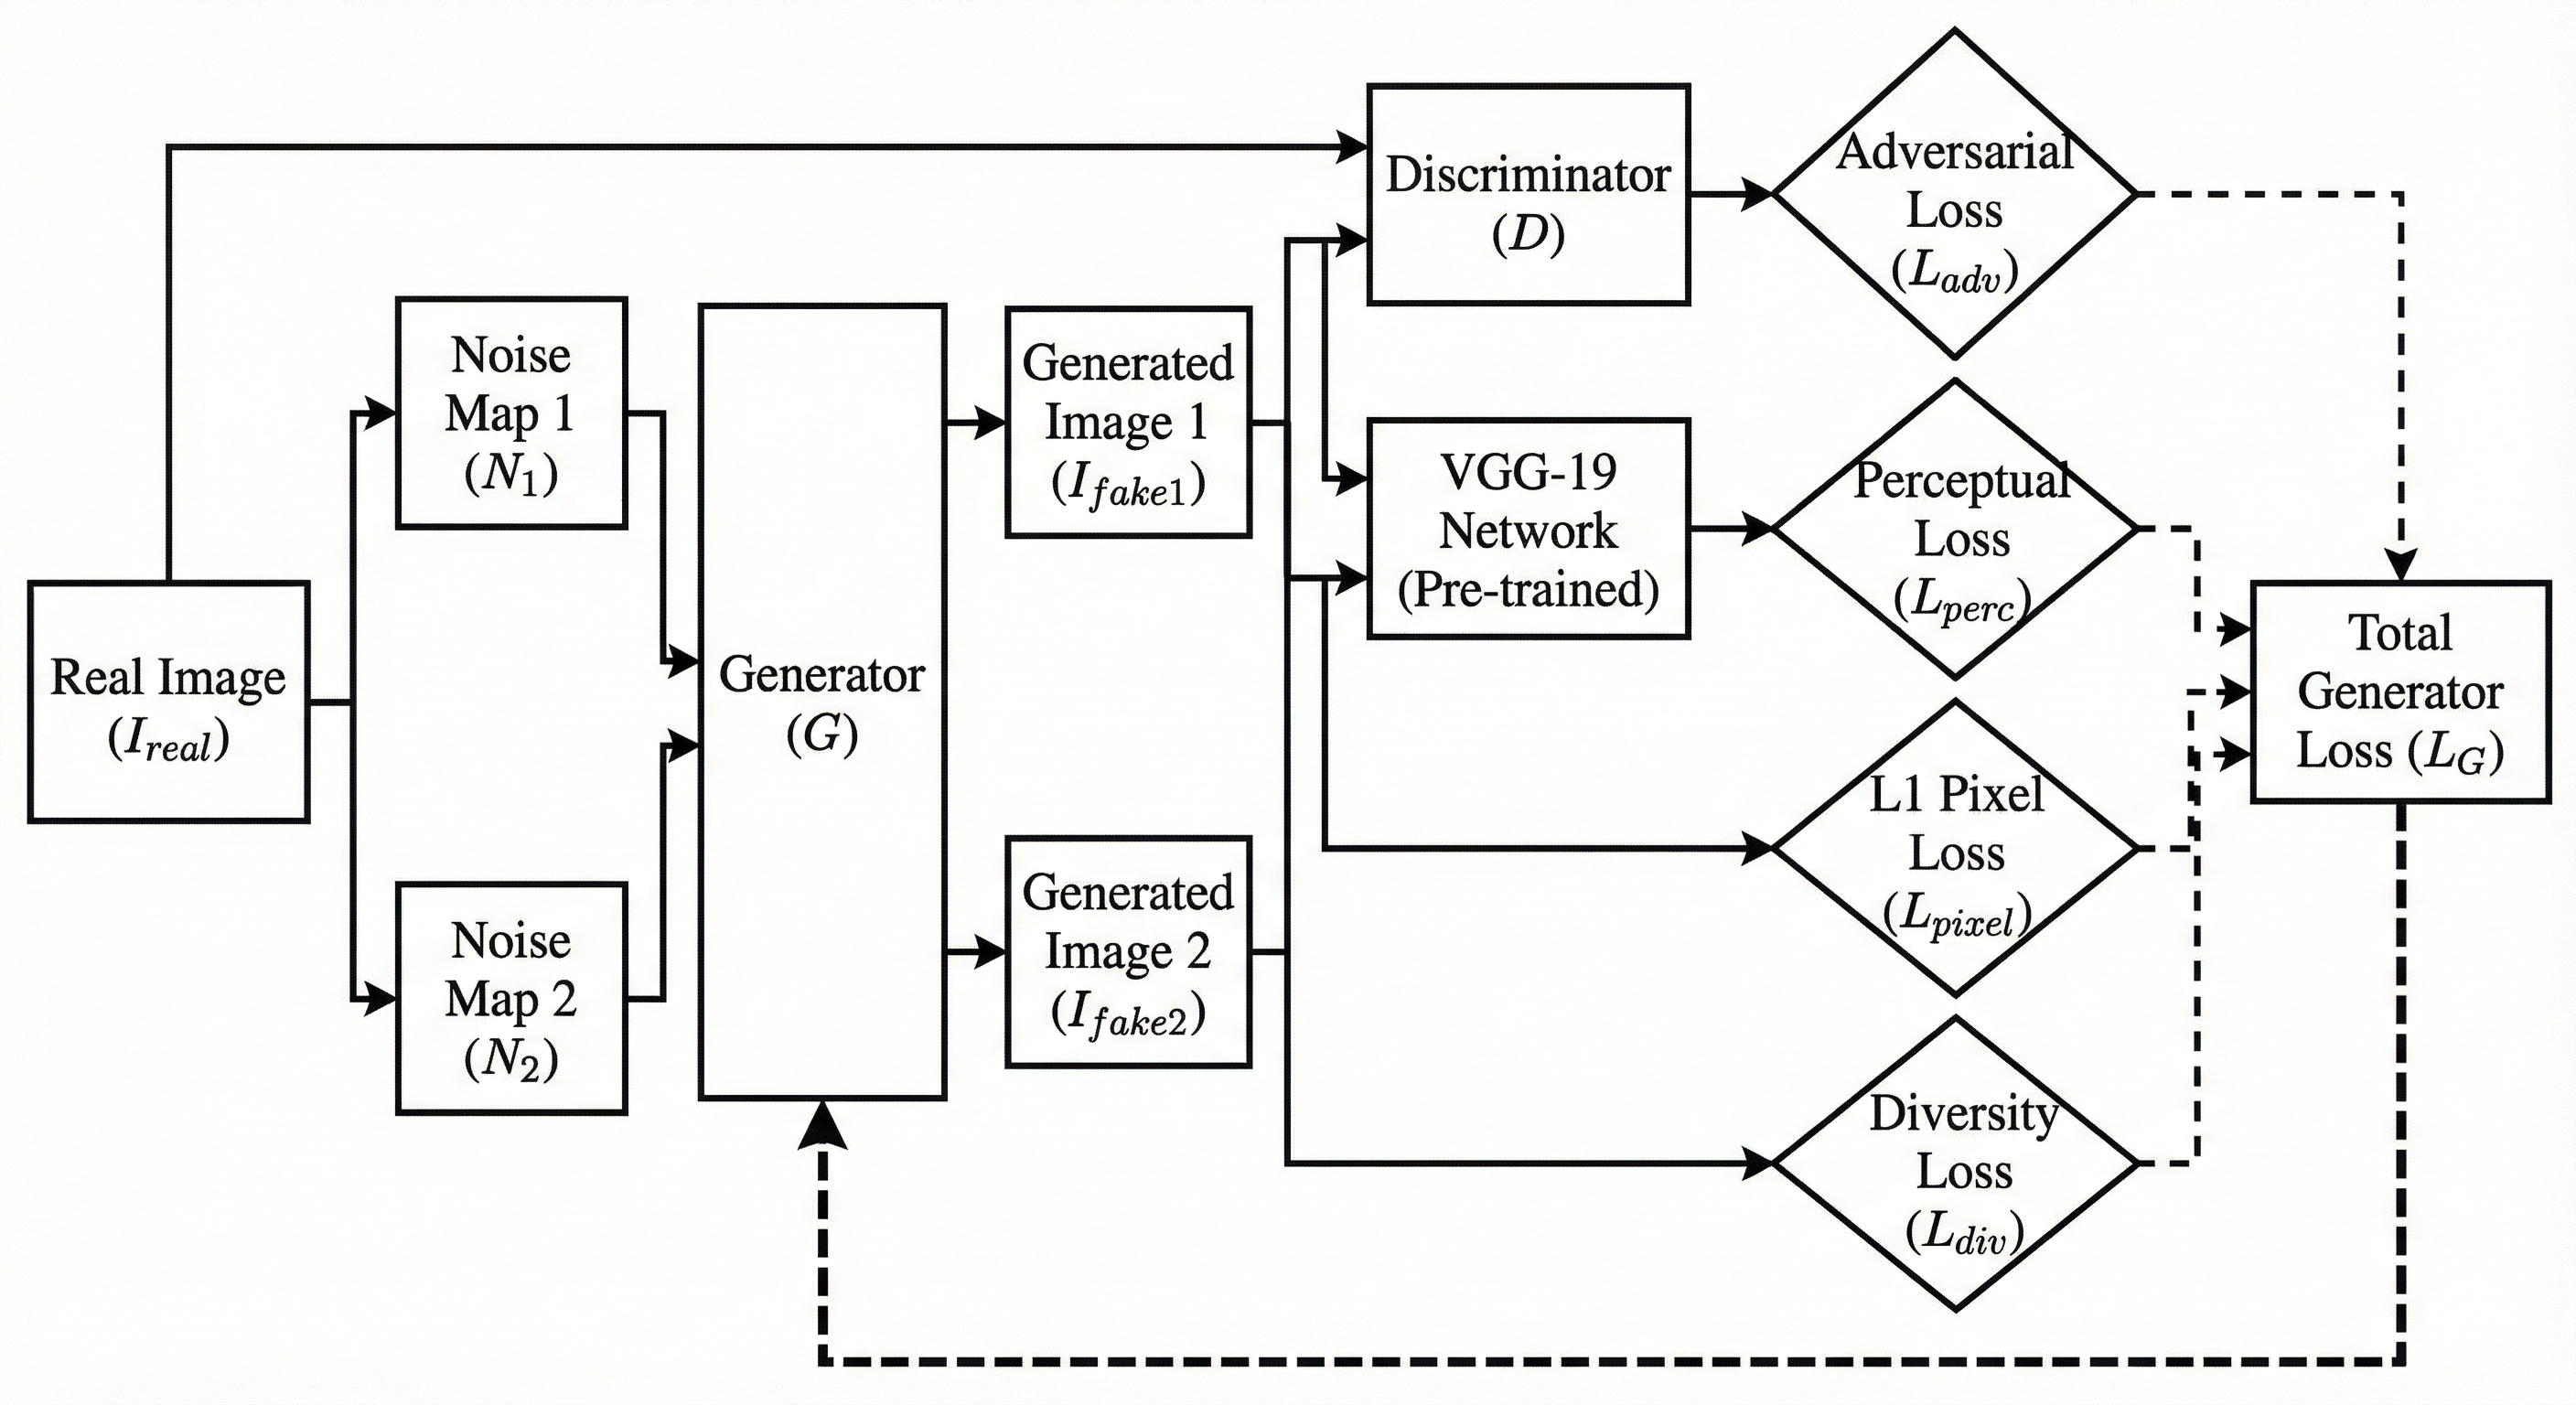
\includegraphics[width=0.5\linewidth]{FaceID_GAN_workflow_diagram.png}
    \caption{FaceID-GAN Architecture Flow Chart}
\end{figure}

First, we perform data augmentation on the RAF-DB facial image dataset. We designed a FaceID-GAN architecture that takes random noise as input and utilizes a generator integrated with a VGG-19 pre-trained network to generate fake images. To address the issue of “Mode Collapse to Identity” where the generator tends to produce images overly similar to the originals to minimize loss, we introduced a diversity loss mechanism. This mechanism ensures that while the generated fake images preserve the original facial expression features (Face ID), they remain visually distinct from the source images. The flowchart of our FaceID-GAN is illustrated in Figure 4. Following the training of the FaceID-GAN model, for which the training loss plot is shown in Figure 5, we utilized it to augment the original RAF-DB, resulting in a dataset five times larger than the original.

\begin{figure}[H]
    \centering
    \includegraphics[width=1\linewidth]{faceid_loss_plot.png}
    \caption{FaceID-GAN Model Training Loss Plot}
\end{figure}

\subsubsection{Facial Geometric Features Extraction}

\begin{figure}[H]
    \centering
    \includegraphics[ width=0.5\linewidth]{MediaPipe_flowchart.png}
    \caption{Facial Geometric Features Extraction Flow Chart}
\end{figure}

We utilized a pre-trained MediaPipe face landmark model \cite{9} to extract the 3D coordinates (x, y, z) of 478 landmarks from the human face. From this comprehensive set, we selected 21 landmarks identified as most critical. Following a standardization process, we perform geometric feature extraction to synthesize these points into 125 highly discriminative geometric attributes. These 125 attributes are categorized into five distinct groups: \textbf{key coordinates} (3D positions of the eyes, nose, mouth, eyebrows, and chin), \textbf{distances} (facial dimensions between landmark pairs, e.g., eye width/height), \textbf{angles} (facial geometry derived from landmark triplets, e.g., eye-bridge angle and mouth angle), \textbf{geometric ratios} (proportional relationships, e.g., eye openness), and \textbf{regional statistics} (metrics including spread, aspect ratio, and centroid positions across nine facial regions covering the eyes, eyebrows, nose, lips, and jaw). Importantly, because these attributes are derived from 3D landmark coordinates, they exhibit inherent robustness to variations in scale and pose after standardizations and geometric feature engineering. Specifically, even when the subject's face is oriented laterally or in a non-frontal pose, the 125 geometric features derived from these 21 key 3D coordinates remain consistent and standardized, ensuring pose invariance. The complete flowchart of our Facial Geometric Features Extraction process is presented in Figure 6.

\subsubsection{ResNet-Like Model for Single-Image FER}

\begin{figure}[H]
    \centering
    \includegraphics[width=0.5\linewidth]{LandmarkClassifier_flowchart.png}
    \caption{ResNet-Like Neural Network Model Architecture}
\end{figure}

Following the extraction of the 125 geometric facial attributes, we designed a customized neural network model based on ResNet’s architecture. This model accepts these geometric attributes as input (input dimension = 125) and was trained using our augmented RAF-DB single-image dataset. The network outputs classification scores for seven emotion categories (output dimension = 7): \textbf{surprise}, \textbf{sadness}, \textbf{neutral}, \textbf{happiness}, \textbf{fear}, \textbf{disgust}, and \textbf{anger}. A softmax function is subsequently applied to these scores to calculate the probability distribution (confidence levels) across the emotions. The category with the highest probability is selected as the final prediction for the single-image FER task, and its confidence level is recorded. The specific architecture of our customized ResNet model is illustrated in Figure 7. After training and hyperparameter tuning, our model achieved an accuracy of 84.55\% on the augmented RAF-DB test set, surpassing the 82.46\% accuracy of the CNN baseline model referenced in previous studies. Compared to processing raw pixel inputs (e.g., 75x75 images), our model is significantly more lightweight, as the feature engineering step reduces the input to just 125 geometric attributes, thereby drastically lowering the data processing load. The detailed training performance of the model is presented in Figure 8.

\begin{figure}[H]
    \centering
    \begin{subfigure}[b]{0.45\linewidth}
        \includegraphics[width=\linewidth]{resnet_loss_plot.png}
        \caption{Training and Validation Loss}
    \end{subfigure}
    \begin{subfigure}[b]{0.45\linewidth}
        \includegraphics[width=\linewidth]{resnet_acc_plot.png}
        \caption{Training and Validation Accuracy}
    \end{subfigure}
    \caption{Training Performance of ResNet-Like Model on Augmented RAF-DB Dataset}
\end{figure}

\subsubsection{Fine-tune Model for Sequential-Image FER}

\begin{figure}[H]
    \centering
    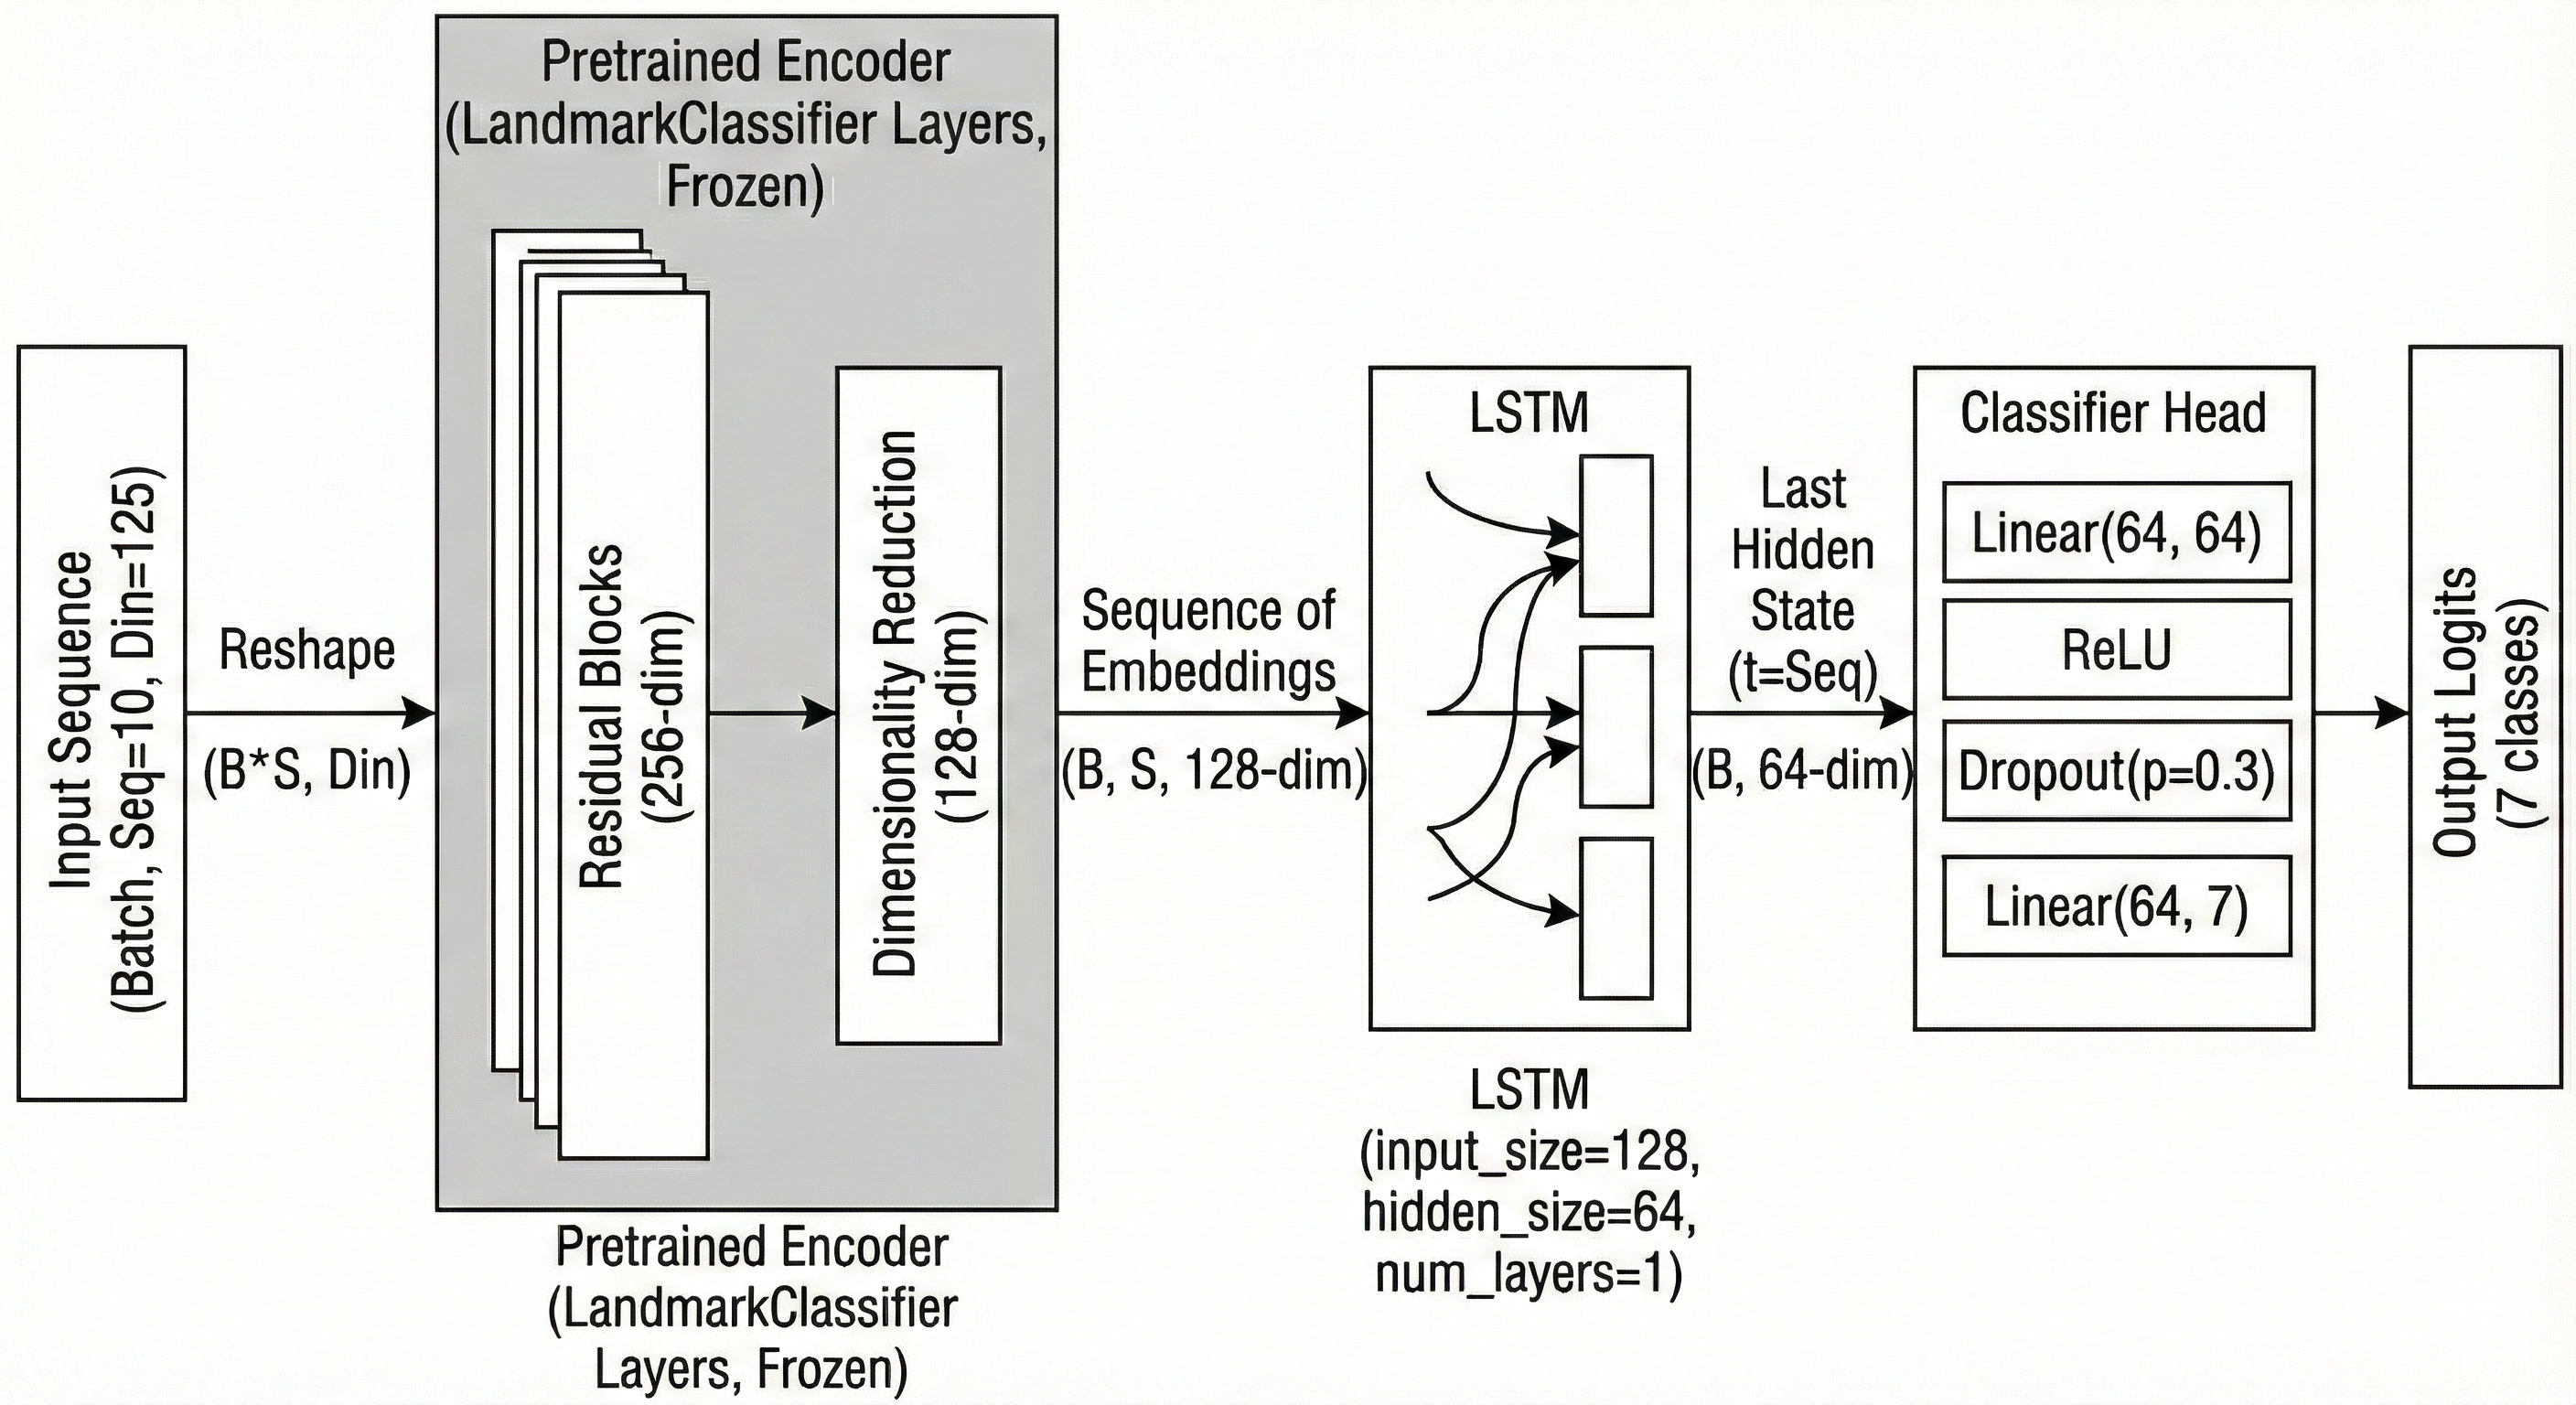
\includegraphics[width=0.5\linewidth]{HybridRNN_flowchart.png}
    \caption{Sequential-Image FER RNN Model Architecture}
\end{figure}

In the previous step, upon achieving a robust single-frame FER model, we effectively established a sophisticated facial geometric feature encoder (hidden layers). To fully leverage this encoder, we initialized our sequential model by loading the pre-trained single-image FER network. Specifically, we removed the final classifier layer while retaining all hidden layers, as they are capable of extracting rich facial information from individual frames. We then introduced an LSTM layer to allow the model to integrate temporal context from the last 10 frames (sequence length = 10) for a complete facial emotion analysis within video or streaming inputs. Finally, two fully connected layers were added to the architecture. The structure of our Sequential-Image FER RNN model is illustrated in Figure 9. Subsequently, we trained this RNN model using the RAVDESS video dataset \cite{8}. Given that our geometric feature encoder (the retained hidden layers) had already demonstrated excellent performance in single-frame FER tasks, we applied a very small learning rate to these layers during training, rather than freezing their parameters entirely. After training and hyperparameter tuning, our model achieved an exceptional accuracy of 97.85\% on the RAVDESS test set \cite{8}. The detailed training performance of the model is shown in Figure 10. This trained RNN model demonstrates high efficiency and accuracy in analyzing human facial emotions during real-time streaming.

\begin{figure}[H]
    \centering
    \begin{subfigure}[b]{0.45\linewidth}
        \includegraphics[width=\linewidth]{rnn_loss_plot.png}
        \caption{Training and Validation Loss}
    \end{subfigure}
    \begin{subfigure}[b]{0.45\linewidth}
        \includegraphics[width=\linewidth]{rnn_acc_plot.png}
        \caption{Training and Validation Accuracy}
    \end{subfigure}
    \caption{Training Performance of RNN Model on RAVDESS Dataset}
\end{figure}


\section{Results}
\subsection{Initial Experiment}
As shown in Figure 1, the baseline model on RAF-DB exhibits a stable convergence in the training split. Using accuracy as an evaluation metric, it reaches a test accuracy of 82.46\%. The qualitative results are provided in Figure 11.

\begin{figure}[H]
    \centering
    \begin{subfigure}[b]{0.3\linewidth}
        \includegraphics[width=\linewidth]{angry_bl.png}
        \caption{Prediction: Angry}
        \label{fig:angry_bl}
    \end{subfigure}
    \begin{subfigure}[b]{0.3\linewidth}
        \includegraphics[width=\linewidth]{disg_bl.png}
        \caption{Prediction: Disgust}
        \label{fig:disg_bl}
    \end{subfigure}
    \begin{subfigure}[b]{0.3\linewidth}
        \includegraphics[width=\linewidth]{happy_bl.png}
        \caption{Prediction: Happy}
        \label{fig:happy_bl}
    \end{subfigure}
    \caption{Sample Predictions from Baseline Model}
\end{figure}

As shown in Figure 3, our pipeline achieves an overall test accuracy of 37. 20\% on RAF-DB when aggregating predictions in the three clarity strata: blurry, moderately blurry and not blurry. In Figure 2, all three clarity-specific models demonstrate gradual convergence in their respective training subsets. Representative visual outputs for our pipeline are shown in Figure 12.

\begin{figure}[H]
    \centering
    \begin{subfigure}[b]{0.3\linewidth}
        \includegraphics[width=\linewidth]{angry_ml.png}
        \caption{Prediction: Angry}
        \label{fig:angry_ml}
    \end{subfigure}
    \begin{subfigure}[b]{0.3\linewidth}
        \includegraphics[width=\linewidth]{disg_ml.png}
        \caption{Prediction: Disgust}
        \label{fig:disg_ml}
    \end{subfigure}
    \begin{subfigure}[b]{0.3\linewidth}
        \includegraphics[width=\linewidth]{happy_ml.png}
        \caption{Prediction: Happy}
        \label{fig:happy_ml}
    \end{subfigure}
    \caption{Sample Predictions from Our Models}
\end{figure}

\subsection{Next-Stage Solution}

\begin{figure}[H]
    \centering
    \includegraphics[width=1\linewidth]{overview_of_the_training_and_inference_pipeline.png}
    \caption{Overview of Training and Inference Pipelines}
\end{figure}

\subsubsection{Data Augmentation: FaceID-GAN}
We applied our pre-trained FaceID-GAN model to the RAF-DB image dataset to perform data augmentation. Specifically, for each original image, the generator generated five additional "fake" images, as illustrated in Figure 14. This strategy expanded the volume of our training data by a factor of five. By introducing increased noise and randomness into the training set, this approach significantly enhances the generalization ability of the trained models.

\begin{figure}[H]
    \centering
    \begin{subfigure}[b]{0.18\linewidth}
        \includegraphics[width=\linewidth]{1.jpg}
    \end{subfigure}
    \begin{subfigure}[b]{0.18\linewidth}
        \includegraphics[width=\linewidth]{2.jpg}
    \end{subfigure}
    \begin{subfigure}[b]{0.18\linewidth}
        \includegraphics[width=\linewidth]{3.jpg}
    \end{subfigure}
    \begin{subfigure}[b]{0.18\linewidth}
        \includegraphics[width=\linewidth]{4.jpg}
    \end{subfigure}
    \begin{subfigure}[b]{0.18\linewidth}
        \includegraphics[width=\linewidth]{5.jpg}
    \end{subfigure}
    \caption{Sample Augmented Images from FaceID-GAN Generator}
\end{figure}

\subsubsection{Facial Geometric Features Extraction}
For all input data, encompassing both single images and video/streaming feeds, we initially employ the Facial Geometric Features Extraction module to process the raw inputs into 125-dimensional geometric feature vectors. This module has proven highly effective in achieving lightweight extraction of critical information from diverse input sources. As the core feature extraction component, it establishes the foundation on which the performance of all our models are based. An example of the output generated by the MediaPipe landmarks extraction model \cite{9} within this module is illustrated in Figure 15.

\begin{figure}[H]
    \centering
    \begin{subfigure}[b]{0.4\linewidth}
        \includegraphics[width=\linewidth]{origin_aug_226488.png}
        \caption{Original Image}
    \end{subfigure}
    \begin{subfigure}[b]{0.4\linewidth}
        \includegraphics[width=\linewidth]{vis_angry_aug_226488.png}
        \caption{Image with 21 Critical 3D Landmarks}
    \end{subfigure}
    \caption{Facial 3D Landmarks Extraction}
\end{figure}

\subsubsection{ResNet-Like Model for Single-Image FER}
Following the model training pipeline depicted in Figure 13(a), we train the single-image FER model on image dataset. As illustrated in Figure 8, the training loss curve exhibited a gradual decline, ultimately achieving excellent convergence while stabilizing at a level slightly higher than the validation loss curve. This behavior indicates that the model has effectively learned from the dataset, a conclusion further supported by the final test accuracy of 84.55\%, which outperforms the 82.46\% test accuracy achieved by our baseline model from paper. 

\subsubsection{Fine-tune Model for Sequential-Image FER}
Following the model training pipeline outlined in Figure 13(b), we trained the sequential-image FER model using the video dataset. As demonstrated in Figure 10, the training loss curve showed a steady decline, ultimately converging perfectly and aligning with the validation loss curve. We achieved a final accuracy of 97.85\% on the video dataset's test set. Furthermore, utilizing the model inferencing pipeline outlined in Figure 13(c), we successfully executed real-time FER tasks by feeding streaming data from a live camera into our trained sequential-image FER RNN model. An example screenshot demonstrating the real-time sequential-image FER application is presented in Figure 16. The red dots represent the target landmarks and the green dots represent the unused landmarks.

\begin{figure}[H]
    \centering
    \includegraphics[width=1\linewidth]{demo_screenshot.png}
    \caption{Sample of Real-Time Sequential-Image FER Application}
\end{figure}


\section{Discussion and Conclusion} 
\subsection{Initial Experiment}
The proposed method demonstrates significant advantages in terms of computational cost. In our initial experiments, using only landmark-based features yields very low inference latency and high efficiency. The landmark extraction itself takes approximately 0.08 seconds per image, and the downstream classifier adds negligible overhead.

Despite a gap in performance, the geometric data proved to be a powerful feature set. Although the landmark-only model underperforms the baseline in accuracy, it relies on only five landmarks. This result indicates that landmark geometry is highly determinative for FER and that there remains substantial headroom for improvement within a landmark-first design.

These findings clarify the necessary direction for our future technical strategy. Increasing the number of extracted landmarks and replacing the landmark extractor with a lower-latency model should be our next move. Depending on forthcoming ablations, in our next-stage solution we need to de-prioritize integrating landmarks into the original baseline and instead pursue a landmark-only approach to achieve a high-efficiency, competitive sequential FER model.

\subsection{Current Limitations}
Despite the improved accuracy of our next-stage solution, our current demo exhibits a strong bias toward predicting "happy" and "angry" emotions. In the learned geometric feature space, many other expressions lie close to these two extremes, so the model usually tends to have higher confidence level on "happy" or "angry" rather than more subtle classes. In addition, our training datasets are collected from professional actors under fixed lighting conditions, where emotions are portrayed in an exaggerated, highly distinguishable manner. This distribution shift makes it harder for the model to detect low-amplitude, everyday emotions in real users, especially in more challenging real-world environments.

\subsection{Future Work}
One key direction is to train on more comprehensive and diverse video datasets for facial emotion recognition. Existing benchmarks are limited in both the range of emotions and the variability of subjects, lighting, and recording conditions, which constrains the model’s ability to generalize to in-the-wild data. Curating or adopting larger, more diverse datasets—especially those featuring non-actors and more naturalistic expressions—could significantly improve robustness. In addition, our current model tends to be over-confident on "happy" and "angry" due to their extreme positions in feature space. As for future work, normalization strategies (e.g., calibrated confidence scaling or feature-space normalization) may be helpful to mitigate this bias, reduce over-confidence on extreme emotions, and encourage more balanced predictions across all classes.







\medskip

\small

\begin{thebibliography}{9}

\bibitem{1}
S. Li, W. Deng, and J. Du, ``Reliable crowdsourcing and deep locality-preserving learning for expression recognition in the wild,'' in \textit{Proc. IEEE Conf. Comput. Vis. Pattern Recognit. (CVPR)}, Honolulu, HI, USA, 2017, pp. 2584--2593.

\bibitem{2}
I. J. Goodfellow, D. Erhan, P. L. Carrier, A. Courville, M. Mirza, B. Hamner, and Y. Bengio, ``Challenges in representation learning: A report on three machine learning contests,'' in \textit{Proc. ICML Workshop Challenges Represent. Learn.}, Atlanta, GA, USA, 2013, pp. 1--10.

\bibitem{3}
M. F. Ali, M. Khatun, and N. A. Turzo, ``Facial emotion detection using neural network,'' \textit{Int. J. Sci. Eng. Res.}, vol. 11, no. 8, pp. 1318--1325, Aug. 2020.

\bibitem{4}
D. Prajapati, ``Balanced RAF-DB dataset (75x75 grayscale),'' Kaggle, 2025. [Online]. Available: \url{https://www.kaggle.com/datasets/dollyprajapati182/balanced-raf-db-dataset-7575-grayscale}

\bibitem{5}
K. Sun \textit{et al.}, ``High-resolution representations for labeling pixels and regions,'' in \textit{Proc. IEEE/CVF Conf. Comput. Vis. Pattern Recognit. (CVPR)}, Seattle, WA, USA, 2020, pp. 7907--7916.

\bibitem{6}
X. Jiang \textit{et al.}, ``DFEW: A large-scale database for recognizing dynamic facial expressions in the wild,'' arXiv preprint arXiv:2008.05924, 2020. [Online]. Available: \url{https://dfew-dataset.github.io/download.html}

\bibitem{7}
S. Stoychev and H. Gunes, ``The effect of model compression on fairness in facial expression recognition,'' in \textit{Pattern Recognition, Computer Vision, and Image Processing. ICPR 2022 Int. Workshops and Challenges}, Montreal, QC, Canada, 2022.

\bibitem{8}
S. R. Livingstone and F. A. Russo, ``The Ryerson Audio-Visual Database of Emotional Speech and Song (RAVDESS),'' \textit{PLoS ONE}, vol. 13, no. 5, p. e0196391, May 2018, doi: 10.5281/zenodo.1188976.

\bibitem{9}
C. Lugaresi \textit{et al.}, ``MediaPipe: A framework for building perception pipelines,'' arXiv preprint arXiv:1906.08172, 2019. [Online]. Available: \url{https://arxiv.org/abs/1906.08172}

\end{thebibliography}

\end{document}